\documentclass{standalone}
\usepackage{tikz}
\usetikzlibrary{patterns, positioning}
\usepackage[sfdefault]{ClearSans} %% option 'sfdefault' activates Clear Sans as the default text font
\usepackage[T1]{fontenc}

\begin{document}
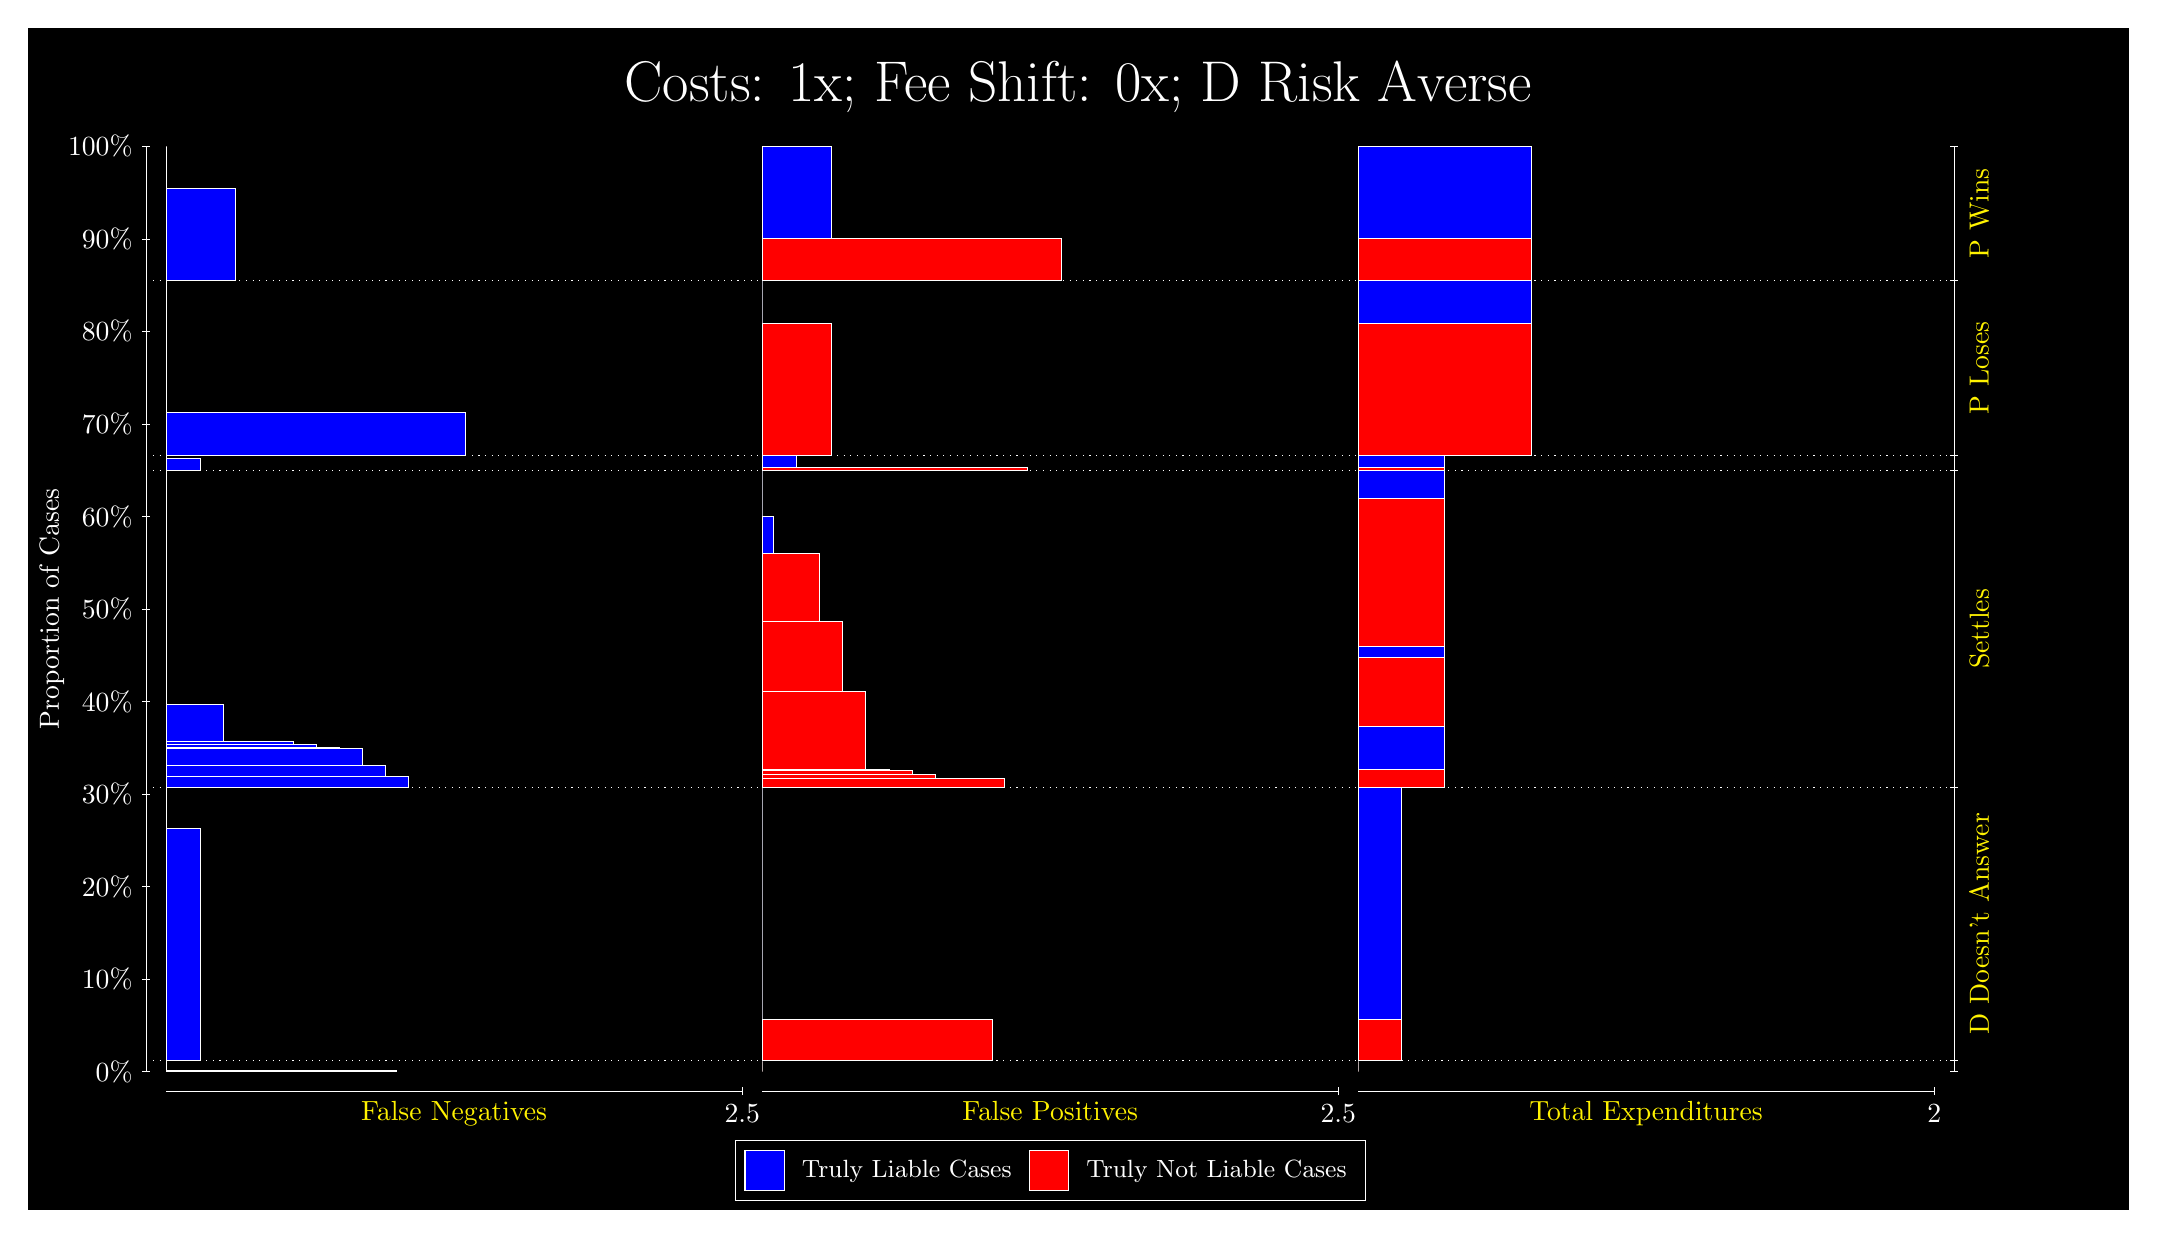
\begin{tikzpicture}
\draw[fill=black] (0,0) rectangle (26.667,15);
\draw[text=white] (0,13.5) rectangle (26.667,15) node[midway] {\huge Costs: 1x; Fee Shift: 0x; D Risk Averse};
\draw[white, very thin] (1.5,1.75) -- (1.5,13.5);
\node[rotate=90, text=white, anchor=center] at (0.3, 7.625) {Proportion of Cases};
\draw[white, very thin] (1.45,1.75) -- (1.55,1.75);
\node[text=white, anchor=east] at (1.45, 1.75) {0\%};
\draw[white, very thin] (1.45,2.925) -- (1.55,2.925);
\node[text=white, anchor=east] at (1.45, 2.925) {10\%};
\draw[white, very thin] (1.45,4.1) -- (1.55,4.1);
\node[text=white, anchor=east] at (1.45, 4.1) {20\%};
\draw[white, very thin] (1.45,5.275) -- (1.55,5.275);
\node[text=white, anchor=east] at (1.45, 5.275) {30\%};
\draw[white, very thin] (1.45,6.45) -- (1.55,6.45);
\node[text=white, anchor=east] at (1.45, 6.45) {40\%};
\draw[white, very thin] (1.45,7.625) -- (1.55,7.625);
\node[text=white, anchor=east] at (1.45, 7.625) {50\%};
\draw[white, very thin] (1.45,8.8) -- (1.55,8.8);
\node[text=white, anchor=east] at (1.45, 8.8) {60\%};
\draw[white, very thin] (1.45,9.975) -- (1.55,9.975);
\node[text=white, anchor=east] at (1.45, 9.975) {70\%};
\draw[white, very thin] (1.45,11.15) -- (1.55,11.15);
\node[text=white, anchor=east] at (1.45, 11.15) {80\%};
\draw[white, very thin] (1.45,12.325) -- (1.55,12.325);
\node[text=white, anchor=east] at (1.45, 12.325) {90\%};
\draw[white, very thin] (1.45,13.5) -- (1.55,13.5);
\node[text=white, anchor=east] at (1.45, 13.5) {100\%};

\draw[white, very thin] (24.457,1.75) -- (24.457,13.5);
\draw[white, very thin] (24.407,1.75) -- (24.507,1.75);
\node[anchor=west] at (24.407, 1.75) {};
\draw[white, very thin] (24.407,1.8957) -- (24.507,1.8957);
\node[anchor=west] at (24.407, 1.8957) {};
\draw[white, very thin] (24.407,5.3566) -- (24.507,5.3566);
\node[anchor=west] at (24.407, 5.3566) {};
\draw[white, very thin] (24.407,9.3867) -- (24.507,9.3867);
\node[anchor=west] at (24.407, 9.3867) {};
\draw[white, very thin] (24.407,9.5777) -- (24.507,9.5777);
\node[anchor=west] at (24.407, 9.5777) {};
\draw[white, very thin] (24.407,11.793) -- (24.507,11.793);
\node[anchor=west] at (24.407, 11.793) {};
\draw[white, very thin] (24.407,13.5) -- (24.507,13.5);
\node[anchor=west] at (24.407, 13.5) {};

\draw[white, very thin, fill=blue] (1.75,1.75) rectangle (4.6775,1.7653);
\draw[white, very thin, fill=red] (1.75,1.7653) rectangle (1.75,1.8957);
\draw[white, very thin, fill=blue] (1.75,1.8957) rectangle (2.1891,4.8341);
\draw[white, very thin, fill=red] (1.75,4.8341) rectangle (1.75,5.3566);
\draw[white, very thin, fill=blue] (1.75,5.3566) rectangle (4.8239,5.4967);
\draw[white, very thin, fill=blue] (1.75,5.4967) rectangle (4.5312,5.6446);
\draw[white, very thin, fill=blue] (1.75,5.6446) rectangle (4.2384,5.8521);
\draw[white, very thin, fill=blue] (1.75,5.8521) rectangle (3.9457,5.8665);
\draw[white, very thin, fill=blue] (1.75,5.8665) rectangle (3.6529,5.9016);
\draw[white, very thin, fill=blue] (1.75,5.9016) rectangle (3.3602,5.9473);
\draw[white, very thin, fill=blue] (1.75,5.9473) rectangle (2.4819,6.4116);
\draw[white, very thin, fill=red] (1.75,6.4116) rectangle (1.75,9.3867);
\draw[white, very thin, fill=blue] (1.75,9.3867) rectangle (2.1891,9.5427);
\draw[white, very thin, fill=red] (1.75,9.5427) rectangle (1.75,9.5777);
\draw[white, very thin, fill=blue] (1.75,9.5777) rectangle (5.5558,10.117);
\draw[white, very thin, fill=red] (1.75,10.117) rectangle (1.75,11.793);
\draw[white, very thin, fill=blue] (1.75,11.793) rectangle (2.6283,12.963);
\draw[white, very thin, fill=red] (1.75,12.963) rectangle (1.75,13.5);
\draw[white, very thin, fill=red] (9.3189,1.75) rectangle (9.3189,1.8804);
\draw[white, very thin, fill=blue] (9.3189,1.8804) rectangle (9.3189,1.8957);
\draw[white, very thin, fill=red] (9.3189,1.8957) rectangle (12.246,2.4182);
\draw[white, very thin, fill=blue] (9.3189,2.4182) rectangle (9.3189,5.3566);
\draw[white, very thin, fill=red] (9.3189,5.3566) rectangle (12.393,5.4734);
\draw[white, very thin, fill=red] (9.3189,5.4734) rectangle (11.515,5.5263);
\draw[white, very thin, fill=red] (9.3189,5.5263) rectangle (11.222,5.5763);
\draw[white, very thin, fill=red] (9.3189,5.5763) rectangle (10.929,5.5842);
\draw[white, very thin, fill=red] (9.3189,5.5842) rectangle (10.929,5.5903);
\draw[white, very thin, fill=red] (9.3189,5.5903) rectangle (10.636,6.5762);
\draw[white, very thin, fill=red] (9.3189,6.5762) rectangle (10.344,7.4647);
\draw[white, very thin, fill=red] (9.3189,7.4647) rectangle (10.051,8.3317);
\draw[white, very thin, fill=blue] (9.3189,8.3317) rectangle (9.4652,8.796);
\draw[white, very thin, fill=blue] (9.3189,8.796) rectangle (9.3189,9.3867);
\draw[white, very thin, fill=red] (9.3189,9.3867) rectangle (12.686,9.4217);
\draw[white, very thin, fill=blue] (9.3189,9.4217) rectangle (9.758,9.5777);
\draw[white, very thin, fill=red] (9.3189,9.5777) rectangle (10.197,11.253);
\draw[white, very thin, fill=blue] (9.3189,11.253) rectangle (9.3189,11.793);
\draw[white, very thin, fill=red] (9.3189,11.793) rectangle (13.125,12.33);
\draw[white, very thin, fill=blue] (9.3189,12.33) rectangle (10.197,13.5);
\draw[white, very thin, fill=red] (16.888,1.75) rectangle (16.888,1.8804);
\draw[white, very thin, fill=blue] (16.888,1.8804) rectangle (16.888,1.8957);
\draw[white, very thin, fill=red] (16.888,1.8957) rectangle (17.437,2.4182);
\draw[white, very thin, fill=blue] (16.888,2.4182) rectangle (17.437,5.3566);
\draw[white, very thin, fill=red] (16.888,5.3566) rectangle (17.986,5.5842);
\draw[white, very thin, fill=blue] (16.888,5.5842) rectangle (17.986,6.1386);
\draw[white, very thin, fill=red] (16.888,6.1386) rectangle (17.986,7.0056);
\draw[white, very thin, fill=blue] (16.888,7.0056) rectangle (17.986,7.1456);
\draw[white, very thin, fill=red] (16.888,7.1456) rectangle (17.986,9.0261);
\draw[white, very thin, fill=blue] (16.888,9.0261) rectangle (17.986,9.3867);
\draw[white, very thin, fill=red] (16.888,9.3867) rectangle (17.986,9.4217);
\draw[white, very thin, fill=blue] (16.888,9.4217) rectangle (17.986,9.5777);
\draw[white, very thin, fill=red] (16.888,9.5777) rectangle (19.083,11.253);
\draw[white, very thin, fill=blue] (16.888,11.253) rectangle (19.083,11.793);
\draw[white, very thin, fill=red] (16.888,11.793) rectangle (19.083,12.33);
\draw[white, very thin, fill=blue] (16.888,12.33) rectangle (19.083,13.5);
\draw[white, dotted] (1.5,1.8957) -- (24.457,1.8957);
\draw[white, dotted] (1.5,5.3566) -- (24.457,5.3566);
\draw[white, dotted] (1.5,9.3867) -- (24.457,9.3867);
\draw[white, dotted] (1.5,9.5777) -- (24.457,9.5777);
\draw[white, dotted] (1.5,11.793) -- (24.457,11.793);
\draw[white, very thin] (1.75,1.5) -- (9.0689,1.5);
\node[text=yellow, anchor=north] at (5.4094, 1.5) {False Negatives};
\draw[white, very thin] (9.0689,1.45) -- (9.0689,1.55);
\node[text=white, anchor=north] at (9.0689, 1.45) {2.5};

\draw[white, very thin] (9.3189,1.5) -- (16.638,1.5);
\node[text=yellow, anchor=north] at (12.978, 1.5) {False Positives};
\draw[white, very thin] (16.638,1.45) -- (16.638,1.55);
\node[text=white, anchor=north] at (16.638, 1.45) {2.5};

\draw[white, very thin] (16.888,1.5) -- (24.207,1.5);
\node[text=yellow, anchor=north] at (20.547, 1.5) {Total Expenditures};
\draw[white, very thin] (24.207,1.45) -- (24.207,1.55);
\node[text=white, anchor=north] at (24.207, 1.45) {2};


\node[text=yellow, centered, rotate=90] at (24.777, 3.6262) {D Doesn't Answer};
\node[text=yellow, centered, rotate=90] at (24.777, 7.3717) {Settles};

\node[text=yellow, centered, rotate=90] at (24.777, 10.685) {P Loses};
\node[text=yellow, centered, rotate=90] at (24.777, 12.646) {P Wins};

\draw (12.978300999999998,1.5) node[draw=none] (baseCoordinate) {};
\begin{scope}[align=center]
        \matrix[scale=0.5, draw=white, below=0.5cm of baseCoordinate, nodes={draw}, column sep=0.1cm]{
            \node[rectangle, draw, minimum width=0.5cm, minimum height=0.5cm, fill=blue] {}; &
            \node[draw=none, font=\small, text=white] (B) {Truly Liable Cases}; &
            \node[rectangle, draw, minimum width=0.5cm, minimum height=0.5cm, fill=red] {}; &
            \node[draw=none, font=\small, text=white] (B) {Truly Not Liable Cases}; \\
            };
\end{scope}

\end{tikzpicture}
\end{document}